% Tipo de documento y paquetes a utilizar.
\documentclass[12pt]{article}
\usepackage[utf8]{inputenc}
% \usepackage{amsmath, amsthm, amsfonts, mathtools} % Paquete para usar más fórmulas y ecuaciones.
\usepackage{graphicx}       % Paquete para usar imágenes y figuras.
\usepackage{geometry}       % Paquete para trabajar con los márgenes del documento.
\usepackage{fancyhdr}       % Paquete para personalizar encabezado y pie de página.
\usepackage{lastpage}       % Paquete para referenciar páginas del documento.
\usepackage{listings}       % Paquete para escribir código de programación.
\usepackage{inconsolata}    % Paquete de tipo de letra consola.
\usepackage{multirow}       % Paquete para combinar filas y columnas en tablas.
\usepackage{array}          % Paquete para trabajar tablas especializadas.
\usepackage{xcolor}         % Paquete básico para agregar color al texto.
\usepackage{float}          % Paquete para utilizar fijación de figuras H.
\usepackage{hyperref}       % Paquete para insertar links en el documento.

% Define colores nuevos
\definecolor{color}{HTML}{E4E4EE}
\definecolor{verde}{HTML}{3C8031}

% Personalización de la fuente para el código.
\lstset{
    language = SQL,                    % Lenguaje con palabras reservadas de este resaltadas.
    basicstyle = \ttfamily\footnotesize,             % Utiliza la fuente tttfamily, en especial el paquete inconsolata.
    frame = single,                     % Quita el marco al cuadro flotante que contiene el código o texto.
    backgroundcolor = \color{color},    % Cambia el color del fondo del marco del código. Utiliza el paquete "xcolor" y define un nuevo color.
    columns = fullflexible,             % Ajusta el cuadro flotante al tamaño del texto del documento.
    breaklines = true,                  % Ajusta el texto dentro del contenedor.
    inputencoding = utf8,               % Admite caracteres del código UTF8.
    extendedchars = true,               % Soporte para caracteres especiales.
    %numbers = left,                    % Agrega número de línea al código (izquierda, sin número y derecha).
    showstringspaces = false,           % Quita los guiones bajos predeterminados de los espacios en cadenas de texto.
    escapebegin = \obeyspaces,          % Complemento de la entrada anterior.
    % rulecolor = \color{red},          % Color del borde del marco del código.
    % numberstyle = \color{red},        % Color de los números en el texto o código.
    % stringstyle = \color{red},        % Color de las cadenas de texto en el texto o código.
    % keywordstyle = \color{red},       % Color de las palabras reservadas en el texto o código.
    % identifierstyle = \color{red},    % Color del texto o código.
    commentstyle = \color{verde},       % Color de los comentarios en el texto o código.
    literate =                          % Acepta los siguientes caracteres especiales fuera de UTF8.
        {á}{{\'a}}1 {é}{{\'e}}1 {í}{{\'i}}1 {ó}{{\'o}}1 {ú}{{\'u}}1
        {Á}{{\'A}}1 {É}{{\'E}}1 {Í}{{\'I}}1 {Ó}{{\'O}}1 {Ú}{{\'U}}1
        {ñ}{{\~n}}1 {Ñ}{{\~N}}1,
}

% Márgenes del documento.
\newgeometry{
    top=2.5cm,     % Superior.
    bottom=2.5cm,  % Inferior.
    outer=2.5cm,   % Parte exterior.
    inner=2.5cm,    % Parte interior.
}

% Personalización de la cabecera y pie de página.
\pagestyle{fancy}
\fancyhf{}
\rhead{Overleaf}                                            % Texto en esquina superior derecha.
\lhead{Apuntes de CSS}                                     % Texto en esquina superior izquierda.
\rfoot{Pagina \thepage \hspace{1pt} de \pageref{LastPage}}  % Texto en esquina inferior derecha (Página n de n).
% Ancho de línea horizontal superior e inferior.
\renewcommand{\headrulewidth}{1pt}
\renewcommand{\footrulewidth}{1pt}

% Datos para la portada del documento.
\title{Apuntes de SQL}
\author{migueluisV}
\date{Realizadas: Marzo 2023}

% Inicio del documento.
\begin{document}

% Cambia los títulos de los índices:
% Content - Índice
% List of Figures - Índice de Figuras
% List of Tables - Índice de Tablas
\renewcommand*\contentsname{Índice}
\renewcommand{\listtablename}{Índice de Tablas}
\renewcommand{\listfigurename}{Índice de Figuras}

% Inserta la portada y los índices.
\maketitle\newpage
\tableofcontents\newpage
\listoffigures\newpage
\listoftables\newpage

\hspace{0.55cm}Este documento se hizo con \href{https://es.overleaf.com/}{\textbf{Overleaf}} y los ejemplos fueron desarrollados y probados dentro del área de código (Code Playground) de \href{https://www.sololearn.com/}{\textbf{Sololearn}}.

% Incluye los archivos que conforman al proyecto.
\section{Conceptos básicos}

\textbf{JavaScript} es uno de los lenguajes de programación más populares, utilizado popularmente para crear sitios web dinámicos e interactivos, pero también es usado para crear aplicaciones de celular, videojuegos, procesamiento de datos y más.


\subsection{Salidas}

\textbf{Dentro de un documento HTML}

Una cosa es desplegar un mensaje en un archivo \textit{.js} y otra en un archivo \textit{.html}, con la función \textbf{document.write()} escribimos una cadena dentro de la etiqueta \textbf{<script>} en un archivo HTML.
\begin{lstlisting}
    <script>
        document.write("Hola mundo.")
    </script>
\end{lstlisting}

Gracias a que estamos escribiendo por medio del lenguaje de etiquetas HTML, podemos aplicar etiquetas del mismo al acabado de nuestro mensaje:
\begin{lstlisting}
    <script>
        <!- El mensaje estará escrito en negrita y cursiva. ->
        document.write("<br><i>Hola mundo.</i></br>")
    </script>
\end{lstlisting}

\textit{Nota}: es recomendable utilizar esta función únicamente para salidas de pruebas u errores.

\textbf{En la consola del buscador}

Para escribir un mensaje en la consola del navegador, utiliza el comando \textbf{console.log()}, el \textbf{texto} que vaya a ser escrito debe estar encerrado \textbf{entre comillas sencillas o dobles} ('texto', "texto").
\begin{lstlisting}
    \console.log("Esto es un mensaje.")
\end{lstlisting}

Este tipo de salida es más utilizada para pruebas y probar el funcionamiento del código, se recomienda esta función contra la mencionada anteriormente.


\subsection{Variables}

Para declarar una variable se utiliza la palabra reservada \textbf{var}:
\begin{lstlisting}
    var x = 10;
\end{lstlisting}

\textit{Nota}: JavaScript diferencia variables con el mismo nombre pero distinta cantidad de variables, "nombre" y "Nombre" son dos variables distintas.

Algunas reglas para la declaración de variables en este lenguaje son:
\begin{enumerate}
    \item El primer carácter de una variable debe ser una letra, \textbf{guión bajo} (\_) o un \textbf{símbolo de dolar} (\$).
    \item El primer carácter de una variable no puede ser un número.
    \item Los nombres de variables no pueden incluir operadores matemáticos o lógicos.
    \item Los nombres de variables no pueden contener espacios en blanco.
    \item Los nombres de variables no pueden contener símbolos especiales (", \#, \%, \&, etc).
\end{enumerate}


\subsection{Comentarios}

Para comentar una sola línea de código se utilizan \textbf{dos diagonales} (\textbf{//}) y para comentar múltiples líneas se utiliza los caracteres \textbf{/*} al inicio de las instrucciones que buscas comentar, y \textbf{*/} al final de las instrucciones.
\begin{lstlisting}
    // Esto es un comentario.
    alert("Mensaje dentro de una alerta.")
    /*
    Esto
    También
    Es
    Un
    Comentario.
    */
\end{lstlisting}


\subsection{Tipos de datos}

En este lenguaje, no es necesario declarar una variable con su tipo de dato, sin embargo, no es una buena práctica declarar una variable con un entero, y algunas instrucciones después, asignarle una cadena de caracteres.
\begin{lstlisting}
    // Declaración de variables.
    var x = 1;
    var y = 1.1;
    var z = 1.1111;
    x = "Esto es una variable"; // Esto no es correcto.
\end{lstlisting}

Podemos utilizar una sola comilla (') o dobles comillas (") para contener un texto dentro de una variable, a su vez, podemos utilizar los escapes \textbackslash " y \textbackslash ' para utilizar dichas comillas dentro de una cadena.
\begin{lstlisting}
    var nombre = "mi nombre es \"mario\"";
    var apellido = 'mi nombre es \'casas\''
    var edad = "mi edad es '21'";
\end{lstlisting}

\textit{Nota}: no es necesario utilizar caracteres de escape de una comilla dentro de dobles comillas, ni dobles comillas dentro de comillas.

Algunos caracteres de escape que podemos utilizan se ven en la \textit{Tabla \ref{tab: 1}}:
\begin{table}[H]
    \begin{center}
        \caption{Caracteres de escape válidos}
        \label{tab: 1}
        \begin{tabular}{c l}
            \hline
            \textbf{Carácter de escape}&\textbf{Función} \\
            \hline
            \textbackslash ' & Una comilla \\
            \textbackslash " & Doble comilla \\
            \textbackslash \textbackslash & Diagonal \\
            \textbackslash n & Salto de línea \\
            \textbackslash r & Posiciona el cursor al inicio de la línea \\
            \textbackslash t & Tabulación \\
            \textbackslash b & Posiciona el cursos un carácter atrás en el texto o consola \\
            \textbackslash f & Genera un salto de página \\
            \hline
        \end{tabular}
    \end{center}
\end{table}

Los \textbf{valores booleanos} son: \textbf{true} y \textbf{false}, el primero para casos positivos o reales, el segundo para valores como 0, null, indefinido o cadenas vacías.


\subsection{Operadores}


\subsubsection{Operadores aritméticos}

La \textit{Tabla \ref{tab: 2}} contiene los operadores aritméticos válidos en este lenguaje:
\begin{table}[H]
    \begin{center}
        \caption{Operadores aritméticos en JavaScript}
        \label{tab: 2}
        \begin{tabular}{c l}
            \hline
            \textbf{Operador}&\textbf{Definición} \\
            \hline
            + & Suma o Concatenación \\
            - & Resta \\
            $\ast$ & Multiplicación \\
            / & División \\
            \% & Modulo (residuo de una división) \\
            ++ & Incremento \\
            -- & Decremento \\
            \hline
        \end{tabular}
    \end{center}
\end{table}

La función \textbf{eval()} toma una cadena que contiene una expresión aritmética y regresa su resultado:
\begin{center}
    \textit{console.log(eval("2 + 2")); // Imprime 4.}
\end{center}

Al igual que en otros lenguajes, JavaScript posee los operadores de incremento y decremento post y pre:
\begin{center}
    \textit{
            var++ (incrementa después de una instrucción) \\
            ++var (incrementa antes de una instrucción) \\
            var-- (decrementa después de una instrucción) \\
            --var (decrementa antes de una instrucción) \\
    }
\end{center}


\subsubsection{Operadores de asignación}

La \textit{Tabla \ref{tab: 3}} contiene los operadores de asignación válidos en este lenguaje:
\begin{table}[H]
    \begin{center}
        \caption{Operadores de asignación en JavaScript}
        \label{tab: 3}
        \begin{tabular}{c l}
            \hline
            \textbf{Operador}&\textbf{Equivalencia} \\
            \hline
            = & x = y \\
            += & x = x + y \\
            -= & x = x - y \\
            *= & x = x * y \\
            /= & x = x / y \\
            \%= & x = x \% y \\
            \hline
        \end{tabular}
    \end{center}
\end{table}

\textit{Nota}: pueden combinarse el uso de varios operadores de asignación en una sola instrucción.


\subsubsection{Operadores de comparación}

La \textit{Tabla \ref{tab: 4}} contiene los operadores de comparación válidos en este lenguaje:
\begin{table}[H]
    \begin{center}
        \caption{Operadores de comparación en JavaScript}
        \label{tab: 4}
        \begin{tabular}{c l}
            \hline
            \textbf{Operador}&\textbf{Definición} \\
            \hline
            == & Igual a \\
            === & Idénticos (iguales o del mismo tipo) \\
            != & No igual a \\
            !== & No idéntico \\
            $>$ & Mayor \\
            $>$= & Mayor igual \\
            $<$ & Menor \\
            $<$= & Menor igual \\
            \hline
        \end{tabular}
    \end{center}
\end{table}

Las comparaciones regresan true o false si son ciertas o no.


\subsubsection{Operadores lógicos y booleanos}

La \textit{Tabla \ref{tab: 5}} contiene los operadores lógicos válidos en este lenguaje:
\begin{table}[H]
    \begin{center}
        \caption{Operadores de comparación en JavaScript}
        \label{tab: 5}
        \begin{tabular}{m{3cm} m{10cm}}
            \hline
            \textbf{Operador}&\textbf{Definición} \\
            \hline
            \&\& & Y. Regresa true si ambas expresiones son verdaderas \\
            $||$ & O. Regresa true si una de las expresiones es verdadera \\
            ! & Negación. Regresa el valor contrario (true o false) al resultado de la expresión \\
            \hline
        \end{tabular}
    \end{center}
\end{table}

Este lenguaje soporta el uso del \textbf{operador ternario}:
\begin{lstlisting}
    var mayorDeEdad = (edad < 18) ? "Muy joven" : "Muy viejo";
\end{lstlisting}

Como vimos, está constituido de una condición, el símbolo de pregunta, su primer valor, dos puntos y el segundo valor; solamente soporta dos valores (true y false), a diferencia de una sentencia if, que puede tener varios \textit{if´s anidados} o \textit{else if}.
\begin{lstlisting}
    variable = (condición) ? valor1 : valor2
\end{lstlisting}

\section{Filtrado de datos}

Anteriormente, seleccionábamos \textbf{todos} los datos de toda una tabla o columna. El comando \textbf{WHERE} permite seleccionar únicamente uno o varios registros que cumplan con una condición. Los operadores pueden ser consultados en la \textit{Tabla \ref{tab: 9}}:
\begin{table}[H]
    \centering
    \caption{Operadores relacionales en SQL}
    \label{tab: 9}
    \begin{tabular}{l l}
        \hline
        \textbf{Operador} & \textbf{Descripción} \\
        \hline
        =           & Igual a \\
        $>$         & Mayor a \\
        $<$         & Menor a \\
        $>$=        & Mayor o igual a \\
        $<$=        & Menor o igual a \\
        $<>$        & Distinto a \\
        !=          & Distinto a  (en algunas versiones de SQL) \\
        \hline
    \end{tabular}
\end{table}

Se pueden utilizar cadenas dentro del filtrado, se especifica el valor de la misma con comillas simples (''), en caso de que el registro contenga una comilla simple (por ejemplo: 'let's'), agregue otra comilla ('let''s'). Las siguientes sentencias son ejemplos de filtrado de datos con operadores lógicos, copie y pegue en su SGBD para poder apreciar los resultados:
\begin{lstlisting}
    SELECT * FROM Personas WHERE edad = 60;
    SELECT * FROM Personas WHERE edad $<>$ 60;
    SELECT * FROM Personas WHERE nombre = 'David';
    SELECT * FROM Personas WHERE edad < 30
\end{lstlisting}

Los comandos \textbf{BETWEEN} y \textbf{AND} sirven para seleccionar un rango de registros resultantes de una sentencia con el comando WHERE, un ejemplo se ve en la \textit{Tabla \ref{tab: 10}}:
\begin{lstlisting}
    SELECT * FROM Personas
    WHERE edad BETWEEN 30 AND 60
\end{lstlisting}
\begin{table}[H]
    \centering
    \caption{Seleccionando un rango de registros con WHERE, BETWEEN y AND}
    \label{tab: 10}
    \begin{tabular}{|l|l|l|l|l|}
        \hline
        \textbf{id} & \textbf{nombre} & \textbf{apellidos} & \textbf{ciudad} & \textbf{edad} \\
        \hline
        2 & David       & Williams  & Los Angeles   & 42 \\
        \hline
        3 & Chloe       & Anderson  & Chicago       & 65 \\
        \hline
        5 & James       & Roberts   & Philadelphia  & 31 \\
        \hline
        7 & Daniel      & Harris    & Los Angeles   & 67 \\
        \hline
        8 & Charlotte   & Walker    & Chicago       & 45 \\
        \hline
    \end{tabular}
\end{table}

\textit{Nota}: los valores límite (30 y 60 para el ejemplo anterior) son incluidos en los registros resultantes.



\section{Condiciones lógicas}

Puede combinar operadores relacionales con operadores lógicos, estos pueden ser consultados en la \textit{Tabla \ref{tab: 11}}:
\begin{table}[H]
    \centering
    \caption{Operadores lógicos en SQL}
    \label{tab: 11}
    \begin{tabular}{m{3cm} m{10cm}}
        \hline
        \textbf{Operador} & \textbf{Descripción} \\
        \hline
        ALL     & Regresa TRUE si todos los valores de una sub-sentencia coinciden con la condición \\
        AND     & Regresa TRUE si las dos condiciones separadas por el operador AND son ciertas \\
        ANY     & Regresa TRUE si alguno de los valores de una sub-sentencia coincide con la condición \\
        BETWEEN & Regresa TRUE si el operador está dentro de un rango de comparación \\
        EXIST   & Regresa TRUE si la sub-sentencia regresa uno o varios registros \\
        IN      & Regresa TRUE si el operador es igual a un item dentro de una lista de expresiones \\
        LIKE    & Regresa TRUE si el operador coincide con el patrón \\
        NOT     & Muestra el contrario o negación de una condición verdadera \\
        OR      & Regresa TRUE si alguna de las dos condiciones separadas por el operador OR son ciertas \\
        SOME    & Regresa TRUE si alguno de los valores de la sub-sentencia coincide con la condición \\
        \hline
    \end{tabular}
\end{table}

Ya se utilizaron los operadores \textbf{BETWEEN} y \textbf{AND} en el tema anterior para conseguir el rango de valores aceptados en la condición. El operador AND permite juntar dos condiciones, si ambas son ciertas, se regresa \textbf{TRUE}. El operador \textbf{OR} sigue la misma lógica, solamente que si alguna de ambas condiciones es cierta, se regresa TRUE. A continuación, ejemplos:
\begin{lstlisting}
    SELECT * FROM Personas
    WHERE ciudad = 'Los Angeles' AND edad = 42;
    SELECT * FROM Personas
    WHERE ciudad = 'Los Angeles' OR ciudad = 'Chicago'
\end{lstlisting}

El operador \textbf{IN} funciona para evitar utilizar varias veces el operador \textbf{OR}, como se ve en el siguiente ejemplo:
\begin{lstlisting}
    SELECT * FROM Personas
    WHERE ciudad
    IN ('Los Angeles', 'Chicago')
\end{lstlisting}

Esta consulta regresa todos los registros que tengan el atributo "ciudad" con los valores "Los Angeles" y "Chicago". Es obligatorio que se utilicen los paréntesis, las comillas simples y separación por comas para todos los valores a utilizar.

Caso contrario, el operador \textbf{NOT} regresará todos los registros con el atributo "ciudad" distinto a "Los Angeles" y "Chicago", es decir, todos los registros contrarios a \textbf{TRUE} o los registros contrarios a los escritos.



\section{Filtros de texto}

Vimos anteriormente que se pueden seleccionar registros en base a la cadena de un atributo, a esta característica se podemos sumar que se pueden recoger registros en base a un patrón. Para lograr este cometido, utilizamos el operador \textbf{LIKE}, en conjunto con los caracteres comodines (Wildcard Characters) y las comillas simples para encerrar el patrón, uno de los más populares es el comodín \%, el cual representa uno o varios caracteres que, para este caso, son ignorados y solamente se toma en cuenta la cadena o caracteres a buscar como patrón, puede consultar más información sobre los comodines en este \href{https://www.w3schools.com/sql/sql_wildcards.asp}{enlace}. Veamos un ejemplo para que se entienda un poco más como se usan estos comodines:
\begin{center}
    \textit{
        '\%sos' ignora los primeros caracteres menos 'sos'. \\
        'be\%' ignora los caracteres siguientes a 'be'. \\
        '\% san \%' ignora los caracteres antes y después de 'san'.
    }
\end{center}

Entonces, con este comodín podemos ignorar \textit{n} cantidad de caracteres y tomar solamente los que nos interesan, siendo esto un patrón que utiliza el operador \textbf{LIKE} para recoger registros con una secuencia de caracteres específicos en una cadena. Veamos varios ejemplos con la tabla de ejemplo que utilizamos y los resultados aparecen en las siguientes tablas:
\begin{lstlisting}
    SELECT * FROM Personas
    WHERE apellidos
    LIKE '\%s'
\end{lstlisting}
\begin{table}[H]
    \centering
    \caption{Seleccionando registros con una "s" al final}
    \label{tab: 12}
    \begin{tabular}{|l|l|l|l|l|}
        \hline
        \textbf{id} & \textbf{nombre} & \textbf{apellidos} & \textbf{ciudad} & \textbf{edad} \\
        \hline
        2 & David       & Williams  & Los Angeles   & 42 \\
        \hline
        4 & Emily       & Adams     & Houston       & 29 \\
        \hline
        5 & James       & Roberts   & Philadelphia  & 31 \\
        \hline
        6 & Andrew      & Thomas    & New York      & 21 \\
        \hline
        7 & Daniel      & Harris    & Los Angeles   & 67 \\
        \hline
    \end{tabular}
\end{table}
\begin{lstlisting}
    SELECT * FROM Personas
    WHERE apellidos
    LIKE '\%a\%'
\end{lstlisting}
\begin{table}[H]
    \centering
    \caption{Seleccionando registros con una "a" en medio}
    \label{tab: 13}
    \begin{tabular}{|l|l|l|l|l|}
        \hline
        \textbf{id} & \textbf{nombre} & \textbf{apellidos} & \textbf{ciudad} & \textbf{edad} \\
        \hline
        2 & David       & Williams  & Los Angeles   & 42 \\
        \hline
        4 & Emily       & Adams     & Houston       & 29 \\
        \hline
        6 & Andrew      & Thomas    & New York      & 21 \\
        \hline
        7 & Daniel      & Harris    & Los Angeles   & 67 \\
        \hline
        8 & Charlotte   & Walker    & Chicago       & 45 \\
        \hline
    \end{tabular}
\end{table}

El primer ejemplo selecciona todos los registros donde el apellido de una persona tenga una "s" al final, mientras que el segundo ejemplo selecciona todos los registros donde el apellido de la persona tenga una "a" en medio.

Este comodín es muy poderoso, podemos usar el comodín \_ para seleccionar únicamente un carácter dentro del patrón, como se ve en la \textit{Tabla \ref{tab: 14}}:
\begin{lstlisting}
    SELECT * FROM Personas
    WHERE apellidos
    LIKE '\_ork'
\end{lstlisting}
\begin{table}[H]
    \centering
    \caption{Seleccionando registros con "ork" al final}
    \label{tab: 14}
    \begin{tabular}{|l|l|l|l|l|}
        \hline
        \textbf{id} & \textbf{nombre} & \textbf{apellidos} & \textbf{ciudad} & \textbf{edad} \\
        \hline
        1 & John        & Smith     & New York      & 24 \\
        \hline
        6 & Andrew      & Thomas    & New York      & 21 \\
        \hline
    \end{tabular}
\end{table}



\section{NULL}

La palabra reservada \textbf{NULL} representa la ausencia de un valor en una tabla. Cuando hacemos un registro dejamos vacío un atributo de la tabla, SQL internamente le asigna NULL a ese valor vacío, NULL es diferente de un espacio en blanco y cero. Podemos comprobar si un registro tiene o no un atributo NULL con la combinación de comandos:
\begin{lstlisting}
    SELECT * FROM Personas
    WHERE apellido IS NULL;
    SELECT * FROM Personas
    WHERE apellido IS NOT NULL;
\end{lstlisting}

\section{Funciones}

SQL posee algunas funciones integradas que nos permite conocer algunos detalles o características de las tablas.


\subsection{COUNT}

La función \textbf{COUNT()} regresa un número entero que representa el total de registros de una tabla, se le puede pasar el carácter asterisco o el nombre de alguna columna para que cuenten los registros:
\begin{lstlisting}
    SELECT COUNT(*) FROM Personas;
    SELECT COUNT(apellidos) FROM PERSONAS;

    // Ambas sentencias regresan 8.
\end{lstlisting}

\textit{Nota}: los valores NULL son ignorados.


\subsection{SUM}

La función \textbf{SUM()} suma todos los valores numéricos (entero o decimal) de una columna, es necesario especificar el nombre de la columna a sumar dentro de los paréntesis de la función:
\begin{lstlisting}
    SELECT SUM(edad) FROM Personas

    // Regresa 324.
\end{lstlisting}

Si se intenta utilizar esta función con textos, el valor de retorno es 0. La suma de valores NULL es NULL. Los valores NULL son ignorados.

Las funciones pueden ser combinadas con condicionales, como por ejemplo:
\begin{lstlisting}
    SELECT SUM(ciudad)
    FROM Personas
    WHERE ciudad = 'New York'

    // Regresa 45.
\end{lstlisting}

La sentencia anterior selecciona los dos registros con el valor "New York" y suma los valores de sus atributos "edad".


\subsection{AVG}

Similar a la función anterior, \textbf{AVG()} regresa el promedio de una columna numérica:
\begin{lstlisting}
    SELECT AVG(edad) FROM Personas

    // Regresa 40.5.
\end{lstlisting}

\textit{Nota}: los valores NULL son ignorados. Si tiene 10 registros de los cuales 5 son NULL, solamente se saca el promedio de los 5 valores que no son NULL.


\subsection{MIN \& MAX}

Las funciones \textbf{MIN()} y \textbf{MAX()} regresan el valor numérico mínimo y máximo de una columna respectivamente. Esta función puede ser utilizada para realizar operaciones aritméticas:
\begin{lstlisting}
    SELECT MIN(edad) FROM Personas;
    SELECT MAX(edad) FROM Personas;

    // Regresan 21 y 67 respectivamente.
\end{lstlisting}


\subsection{UPPER}

Vimos que las funciones anteriores simplemente regresan un valor, sin embargo, otras funciones pueden regresar una columna nueva de una tabla origen, un ejemplo de estas funciones es \textbf{UPER()}, la cual genera una columna con el nombre de la función como nombre y los caracteres de una columna original en mayúsculas, como se ve en la \textit{Tabla \ref{tab: 15}}:
\begin{lstlisting}
    SELECT UPPER(nombre) FROM Personas
\end{lstlisting}
\begin{table}[H]
    \centering
    \caption{Creando una columna personalizada con UPPER}
    \label{tab: 15}
    \begin{tabular}{|l|}
        \hline
        \textbf{upper} \\
        \hline
        JOHN \\
        DAVID \\
        CHLOE \\
        EMILY \\
        JAMES \\
        ANDREW \\
        DANIEL \\
        CHARLOTTE \\
        \hline
    \end{tabular}
\end{table}

Si buscamos generar esta columna con otro nombre que no sea el nombre de la función, podemos utilizar el comando AS, seguido del nuevo nombre, como se ve en la \textit{Tabla \ref{tab: 16}}:
\begin{lstlisting}
    SELECT UPPER(nombre) AS nombre_mayus
    FROM Personas
\end{lstlisting}
\begin{table}[H]
    \centering
    \caption{Creando una columna personalizada con nuevo nombre con UPPER}
    \label{tab: 16}
    \begin{tabular}{|l|}
        \hline
        \textbf{nombre\_mayus} \\
        \hline
        JOHN \\
        DAVID \\
        CHLOE \\
        EMILY \\
        JAMES \\
        ANDREW \\
        DANIEL \\
        CHARLOTTE \\
        \hline
    \end{tabular}
\end{table}

En el caso anterior, el nombre no tiene espacios en blanco, en caso de querer utilizarlos, el nombre de la columna debe estar encerrado en comillas simples. Si desea crear más de una columna personalizada en una sola sentencia, sepárelas con comas:
\begin{lstlisting}
    SELECT UPPER(nombre) AS 'Nombre mayus', edad + 1 AS Edad_Mas_Uno
    FROM Personas
\end{lstlisting}

La sentencia anterior crea dos columnas personalizadas, utilizando una operación aritmética en la segunda para crear una columna con la edad de las personas más 1.



\section{Sub-secuencias}

Podemos utilizar sub-secuencias dentro de otra para obtener registros, estas sub-secuencias deben estar siempre encerradas entre paréntesis, como vemos en la \textit{Tabla \ref{tab: 17}}:
\begin{lstlisting}
    SELECT * FROM Personas
    WHERE edad >
        (SELECT AVG(edad) FROM Personas)
\end{lstlisting}
\begin{table}[H]
    \centering
    \caption{Seleccionando edades mayor al promedio con una sub-secuencia}
    \label{tab: 17}
    \begin{tabular}{|l|l|l|l|l|}
        \hline
        \textbf{id} & \textbf{nombre} & \textbf{apellidos} & \textbf{ciudad} & \textbf{edad} \\
        \hline
        2 & David       & Williams  & Los Angeles   & 42 \\
        \hline
        3 & Chloe       & Anderson  & Chicago       & 65 \\
        \hline
        7 & Daniel      & Harris    & Los Angeles   & 67 \\
        \hline
        8 & Charlotte   & Walker    & Chicago       & 45 \\
        \hline
    \end{tabular}
\end{table}



\section{Agrupaciones}

El comando \textbf{GROUP BY} permite agrupar valores de columnas o atributos duplicados en distintos registros en uno solo, de tal forma que el resultado final de la sentencia muestra solo una vez el valor del atributo duplicado. Veamos el siguiente ejemplo en la \textit{Tabla \ref{tab: 18}} para que podamos visualizarlo de mejor manera:
\begin{lstlisting}
    SELECT ciudad, COUNT(*) AS c
    FROM Personas
    GROUP BY ciudad
    ORDER BY c ASC
\end{lstlisting}
\begin{table}[H]
    \centering
    \caption{Agrupando valores de atributos con GROUP BY}
    \label{tab: 18}
    \begin{tabular}{|l|l|}
        \hline
        \textbf{ciudad} & \textbf{c} \\
        \hline
        Houston         & 1 \\
        \hline
        Philadelphia    & 1 \\
        \hline
        Los Angeles     & 2 \\
        \hline
        Chicago         & 2 \\
        \hline
        New York        & 2 \\
        \hline
    \end{tabular}
\end{table}

Sabemos que tenemos tres usuarios que tienen el valor "New York", "Los Angeles" y "Chicago" respectivamente, por lo que estos valores están duplicados, en el ejemplo anterior seleccionamos la columna "ciudad" y, en vez de desplegar todos los valores de esta columna (incluso los duplicados), utilizamos el comando \textbf{GROUP BY} para agrupar los valores duplicados en uno, y añadimos el conteo de valores duplicados en una nueva columna personalizada nombrada "c".

Cuando se utiliza este comando, se seleccionan únicamente las columnas a agrupar, cada función que utilicemos en nuestra sentencia será aplicada al grupo, es decir:
\begin{lstlisting}
    SELECT [columna a agrupar 1], ..., [columna a agrupar n] [FUNCIÓN]
    ...
    GROUP BY [columna a agrupar 1], ..., [columna a agrupar n]
\end{lstlisting}

Si queremos agregar otra columna a trabajar en el comando \textbf{GROUP BY} tendremos un error, solamente se utilizan las columnas seleccionadas tanto en el \textit{SELECT} com en \textit{GROUP BY}.

El comando \textbf{HAVING} es como el comando \textit{WHERE}, pero aplicado a los grupos, retomemos el último ejemplo y veamos el nuevo resultado en la \textit{Tabla \ref{tab: 19}}:
\begin{lstlisting}
    SELECT ciudad, COUNT(*) AS c
    FROM Personas
    GROUP BY ciudad
    HAVING COUNT(*) > 1
    ORDER BY c ASC
\end{lstlisting}
\begin{table}[H]
    \centering
    \caption{Agrupando valores de atributos con GROUP BY y HAVING}
    \label{tab: 19}
    \begin{tabular}{|l|l|}
        \hline
        \textbf{ciudad} & \textbf{c} \\
        \hline
        Los Angeles     & 2 \\
        \hline
        Chicago         & 2 \\
        \hline
        New York        & 2 \\
        \hline
    \end{tabular}
\end{table}

Agrega la condición de que se desplieguen solamente los grupos con más de una persona habitando en las respectivas ciudades. Aclarando: \textit{WHERE filtra los registros de una sentencia previo a agruparlos, HAVING filtra los grupos}.

\section{Manejo de tablas}


\subsection{Creación de una tabla}

Hasta ahora, siempre manejábamos una sola tabla propuesta por nosotros, sin embargo, el mundo real requiere que el desarrollador cree y manipule sus propias tablas, recodemos nuevamente que las tablas están constituidas por columnas (atributos) y filas (registros). Las columnas de la tabla "Personas" contiene solamente dos tipos de datos, cadena y número entero, la \textit{Tabla \ref{tab: 20}} contiene el resto de tipos de datos disponibles para la creación de columnas en tablas:
\begin{table}[H]
    \centering
    \caption{Tipos de datos disponibles en SQL}
    \label{tab: 20}
    \begin{tabular}{m{4cm} m{9cm}}
        \hline
        \textbf{Nombre} & \textbf{Descripción} \\
        \hline
        INT             & Número entero positivo o negativo \\
        FLOAT           & Número decimal positivo o negativo \\
        DOUBLE          & Como \textit{FLOAT}, pero con mayor rango de valores decimales disponibles \\
        DATE            & Una fecha en formato YYYY-MM-DD \\
        DATETIME        & Una fecha y hora que está en formato YYYY-MM-DD HH:MM:SS \\
        TIMESTAMP       & Una marca de tiempo, calculada desde la medianoche del primero de enero de 1970 \\
        TIME            & Una hora en formato en HH:MM:SS \\
        VARCHAR(largo)  & Una cadena variable con largo definido dentro de los paréntesis \\
        TEXT            & Una cadena muy larga \\
        \hline
    \end{tabular}
\end{table}

A la hora de crear la tabla, debes especificar el tipo de dato que almacenará cada columna, por lo que debes pensar qué tipo de datos almacenarás para que corresponda con el tipo de dato asignado. Veamos la sintaxis para crear una tabla:
\begin{lstlisting}
    CREATE TABLE Clientes (
        id INT,
        firstname VARCHAR(128),
        lastname VARCHAR(128),
        salary INT,
        city VARCHAR(128)
    );
\end{lstlisting}

Como se puede ver, las columnas que conformarán la tabla van encerradas entre paréntesis, separados por una coma y el tipo de dato se separa del nombre de la columna por un espacio, además, el tipo \textit{VARCHAR} recibe el largo del dato a almacenar dentro de paréntesis también.

Si requerimos que, al momento de crear una tabla, se le asigne un valor predeterminado a una de las tablas, se puede utilizar el comando \textbf{DEFAULT}:
\begin{lstlisting}
    CREATE TABLE Clientes (
        id INT,
        firstname VARCHAR(128),
        lastname VARCHAR(128),
        salary INT DEFAULT 0,
        city VARCHAR(128)
    );
\end{lstlisting}

Este comando va enseguida del tipo de dato y el valor va enseguida del comando, al ejecutar esta sentencia, se creará la tabla y todo registro nuevo en la misma tendrá el valor predeterminado de 0 (en caso de que no se le agregue un valor a la columna "salary"). Puede crear una tabla con múltiples valores predeterminados.

Si requerimos que todo registro, al momento de hacer un registro en una tabla, se llenen todos los campos de la misma, podemos utilizar el comando \textbf{NULL} y \textbf{NOT NULL}:
\begin{lstlisting}
    CREATE TABLE Clientes (
        id INT NOT NULL,
        firstname VARCHAR(128) NOT NULL,
        lastname VARCHAR(128),
        salary INT NOT NULL,
        city VARCHAR(128)
    );
\end{lstlisting}

Ahora la tabla "Clientes" requiere obligatoriamente que los campos "id", "firstname" y "salary" sean llenados para el correcto registro.


\subsection{Actualización de una tabla}

El comando \textbf{ALTER TABLE} sirve para agregar, eliminar y modificar una columna en una tabla existe. Añadiremos las columnas "ex1" y "ex2" a la tabla "Clientes" con el comando \textbf{ADD}:
\begin{lstlisting}
    ALTER TABLE Clientes
    ADD ex1 TEXT,
    ADD ex2 TEXT;
\end{lstlisting}

Todos los registros existentes recibirán un valor predeterminado en estas nuevas columnas, el cual es \textbf{NULL}. Note que enseguida del comando \textit{ADD} va el nombre de la columna y su tipo de dato, separados por un espacio. Agregar múltiples columnas en una sentencia indica que cada columna debe separarse por comas. Ahora eliminaremos la columna "ex2" con los comandos \textbf{DROP COLUMN}:
\begin{lstlisting}
    ALTER TABLE Clientes
    DROP COLUMN ex2
\end{lstlisting}

Se borrará la columna y todos los datos almacenados en ella. También podemos cambiar el nombre de una columna existente o el nombre de la tabla con los comandos \textbf{RENAME} y \textbf{TO}:
\begin{lstlisting}
    ALTER TABLE Clientes
    RENAME ex1 TO example1;

    ALTER TABLE Clientes
    RENAME TO Clients;
\end{lstlisting}

El aspecto final de la tabla "Clientes" es el siguiente (\textit{Tabla \ref{tab: 21}}) después de las actualizaciones:
\begin{table}[H]
    \centering
    \caption{Aspecto de la tabla "Clientes" después de varios cambios}
    \label{tab: 21}
    \begin{tabular}{|l|l|l|l|l|}
        \hline
        \textbf{id} & \textbf{firstname} & \textbf{lastname} & \textbf{salary} & \textbf{city} \\
        \hline
    \end{tabular}
\end{table}


\subsection{Eliminación de una tabla}

El comando \textbf{DROP TABLE} permite borrar toda una tabla y su contenido, eliminaremos una tabla imaginaria "People" simplemente para mostrar la sintaxis de la sentencia:
\begin{lstlisting}
    DROP TABLE People
\end{lstlisting}



\section{Manejo de datos}


\subsection{Inserción de registros}

El comando \textbf{INSERT} crea un registro dentro de una tabla, vacía o con registros previos:
\begin{lstlisting}
    INSERT INTO Personas
    VALUES (9,'Mike','Towers','Houston',39)
\end{lstlisting}

Este comando va acompañado del comando \textbf{INTO}, los valores que se vayan a registrar dentro de la tabla van encerrados dentro de paréntesis y son separados por comas, los valores que sean tipo cadena son contenidos dentro de comillas simples (''), los valores numéricos no requieren estas comillas. Asegúrese de que los valores a ingresar estén en el mismo orden de las columnas de la tabla.

El ejemplo anterior es la versión corta de la sentencia de inserción, pero podemos especificar a que columna va a insertarse un registro:
\begin{lstlisting}
    INSERT INTO Personas (id,nombre,apellidos,ciudad,edad)
    VALUES (10,'Steve','Jobs','Philadelphia',41)
\end{lstlisting}

De esta forma, podemos escribir el código evitando escribir los valores a registrar en una columna que no le corresponde. Con esta sintaxis, podemos insertar valores a ciertas columnas únicamente, para que los valores predeterminados se inserten en el registro:
\begin{lstlisting}
    INSERT INTO Clientes (id,firstname,lastname,city)
    VALUES (1,'Mario','España','CDMX')
\end{lstlisting}

Para este ejemplo, retomamos el último aspecto de la tabla "Clientes" que estuvimos creando y modificando en la sección anterior, aquella que tiene el valor 0 como predeterminado para la columna "salary", es por ello que la omitimos en este ejemplo de inserción, quedando el resultado en la \textit{Tabla \ref{tab: 22}}:
\begin{table}[H]
    \centering
    \caption{Inserción de registros en una tabla}
    \label{tab: 22}
    \begin{tabular}{|l|l|l|l|l|}
        \hline
        \textbf{id} & \textbf{firstname} & \textbf{lastname} & \textbf{salary} & \textbf{city} \\
        \hline
        1 & Mario & España & 0 & CDMX \\ 
        \hline
    \end{tabular}
\end{table}

\textit{Nota}: si no escribe un valor para una tabla que es de rellenado obligatorio y no tiene un valor predeterminado, la sentencia \textit{INSERT INTO} lanzará un error.

Si deseamos insertar varios registros en una misma sentencia, simplemente separe cada registro por comas y vea el resultado en la \textit{Tabla \ref{tab: 23}}:
\begin{lstlisting}
    INSERT INTO Clientes (id,firstname,lastname,city)
    VALUES
    (2,'Arnulfo','Rodriguez',500.99,'BCS'),
    (3,'Christopher','Robin',1999.87,'EDOMEX');
\end{lstlisting}
\begin{table}[H]
    \centering
    \caption{Múltiple inserción de registros en una tabla}
    \label{tab: 23}
    \begin{tabular}{|l|l|l|l|l|}
        \hline
        \textbf{id} & \textbf{firstname} & \textbf{lastname} & \textbf{salary} & \textbf{city} \\
        \hline
        1 & Mario       & España    & 0         & CDMX \\ 
        \hline
        2 & Arnulfo     & Rodriguez & 500.99    & BCS \\
        \hline
        3 & Christopher & Robin     & 1999.87   & EDOMEX \\
        \hline
    \end{tabular}
\end{table}


\subsection{Actualización de registros}

El comando \textbf{UPDATE} actualiza los datos de un registro dentro de una tabla:
\begin{lstlisting}
    UPDATE Clientes
    SET salary = 2010.56
    WHERE id = 2
\end{lstlisting}

La actualización de registros dependen de una condición a la cual aplicarle las modificaciones, en el caso anterior se le aplica al registro que tiene un "id" de 2, pero se puede aplicar una condición que afecte a más de un registro (\textbf{si omite la condicional, todos los registros sufrirán la modificación}).

Como con la inserción, podemos actualizar múltiples datos separándolos por coma:
\begin{lstlisting}
    UPDATE Clientes
    SET
    salary = 2210.56,
    city = 'BC'
    WHERE id = 2
\end{lstlisting}

Quedando la tabla "Clientes" de la siguiente manera (\textit{Tabla \ref{tab: 24}}) después de las inserciones y actualizaciones:
\begin{table}[H]
    \centering
    \caption{Actualización de un registro en una tabla}
    \label{tab: 24}
    \begin{tabular}{|l|l|l|l|l|}
        \hline
        \textbf{id} & \textbf{firstname} & \textbf{lastname} & \textbf{salary} & \textbf{city} \\
        \hline
        1 & Mario       & España    & 0         & CDMX \\ 
        \hline
        2 & Arnulfo     & Rodriguez & 2210.56    & BC \\
        \hline
        3 & Christopher & Robin     & 1999.87   & EDOMEX \\
        \hline
    \end{tabular}
\end{table}


\subsection{Eliminación de registros}

El comando \textbf{DELETE} elimina los registros dentro de una tabla:
\begin{lstlisting}
    DELETE FROM Personas
    WHERE id = 10
\end{lstlisting}

Tenga cuidado con la condicional, el caso anterior borra el registro que tiene el atributo "id" igual a 10, si pone una condicional que afecte a más de un registro, todos ellos serán eliminados. La tabla "Personas" queda de la siguiente manera (\ref{tab: 25}) después de las inserciones y eliminación:
\begin{table}[H]
    \centering
    \caption{Aspecto de la tabla "Personas" después de varios cambios}
    \label{tab: 25}
    \begin{tabular}{|l|l|l|l|l|}
        \hline
        \textbf{id} & \textbf{nombre} & \textbf{apellidos} & \textbf{ciudad} & \textbf{edad} \\
        \hline
        1 & John        & Smith     & New York      & 24 \\
        \hline
        2 & David       & Williams  & Los Angeles   & 42 \\
        \hline
        3 & Chloe       & Anderson  & Chicago       & 65 \\
        \hline
        4 & Emily       & Adams     & Houston       & 29 \\
        \hline
        5 & James       & Roberts   & Philadelphia  & 31 \\
        \hline
        6 & Andrew      & Thomas    & New York      & 21 \\
        \hline
        7 & Daniel      & Harris    & Los Angeles   & 67 \\
        \hline
        8 & Charlotte   & Walker    & Chicago       & 45 \\
        \hline
        9 & Mike        & Towers    & Houston       & 39 \\
        \hline
    \end{tabular}
\end{table}

A este conjunto de operaciones de creación, lectura, actualización y eliminación de registros se le conoce como \textbf{CRUD} (Create, Read, Update \& Delete).

\section{Más funciones}

Para continuar con los siguientes temas, el nuevo aspecto de la tabla "Personas" aparece en la \textit{Tabla \ref{tab: 26}}:
\begin{table}[H]
    \centering
    \caption{Tabla "Personas" re acondicionada}
    \label{tab: 26}
    \begin{tabular}{|l|l|l|l|l|}
        \hline
        \textbf{id} & \textbf{nombre} & \textbf{apellidos} & \textbf{ciudad} & \textbf{edad} \\
        \hline
        1 & John        & Smith     & New York      & 24 \\
        \hline
        2 & David       & Williams  & Los Angeles   & 42 \\
        \hline
        3 & Chloe       & Anderson  & Chicago       & 65 \\
        \hline
        4 & Emily       & Adams     & Houston       & \textit{NULL} \\
        \hline
        5 & James       & Roberts   & Philadelphia  & 31 \\
        \hline
        6 & Andrew      & Thomas    & New York      & 21 \\
        \hline
        7 & Daniel      & Harris    & New York      & 67 \\
        \hline
        8 & Charlotte   & Walker    & Chicago       & \textit{NULL} \\
        \hline
        9 & Samuel      & Clark     & San Diego     & \textit{NULL} \\
        \hline
        10 & Anthony    & Young     & Los Angeles   & 52 \\
        \hline
    \end{tabular}
\end{table}


\subsection{De cadenas}

Vimos que SQL posee algunas funciones especiales que permiten realizar conteos u operaciones a las columnas y su contenido, la \textit{Tabla \ref{tab: 27}} contiene más funciones, enfocadas a las cadenas de texto, puede consultar el resto de funciones en este \href{https://www.tutorialspoint.com/sql/sql-string-functions.htm}{enlace}:
\begin{table}[H]
    \centering
    \caption{Funciones para cadenas}
    \label{tab: 27}
    \begin{tabular}{m{6cm} m{8cm}}
        \hline
        \textbf{Función} & \textbf{Descripción} \\
        \hline
        CONCAT(c1, c2, ..., c\textit{n})        & Une dos o más cadenas o datos de distintas columnas \\
        LOWER(columna)                          & Convierte todas las cadenas de una columna a minúsculas \\
        \parbox{5cm}{SUBSTRING(columna,\\comienzo, fin)}       & Extrae una subcadena de una cadena, es decir, de todos los datos de una columna \\
        \parbox{5cm}{REPLACE(columna,\\a-remplazar, remplazo)} & Remplaza una cadena por otra en todos los datos de una columna \\
        LENGTH(cadena)                          & Regresa el total de caracteres de una cadena \\
        FORMAT(numero, decimales)               & Regresa un número decimal con cierta cantidad de decimales \\
        \hline
    \end{tabular}
\end{table}

Puede estas funciones con las tablas mostradas en este documento para ver los resultados. Además, podemos utilizar funciones en conjunto:
\begin{lstlisting}
    SELECT CONCAT(
        SUBSTRING(nombre, 1, 1),
        '. ',
        UPPER(apellidos)) AS name
    FROM Personas
\end{lstlisting}

La sentencia anterior toma la primer letra de cada registro de la columna "nombre" y las combina con cada registro de la columna "apellidos", todo en mayúsculas, quedando el resultado de la siguiente manera (\textit{Tabla \ref{tab: 28}}):
\begin{table}[H]
    \centering
    \caption{Uso de varias funciones en una sola sentencia}
    \label{tab: 28}
    \begin{tabular}{|l|}
        \hline
        \textbf{name} \\
        \hline
        J. SMITH \\
        \hline
        D. WILLIAMS \\
        \hline
        C. ANDERSON \\
        \hline
        E. ADAMS \\
        \hline
        J. ROBERTS \\
        \hline
        A. THOMAS \\
        \hline
        D. HARRIS \\
        \hline
        C. WALKER \\
        \hline
        S. CLARK \\
        \hline
        A. YOUNG \\
        \hline
    \end{tabular}
\end{table}



\subsection{Agregación y matemáticas}

Ya hay punto en ese documento referente a las funciones matemáticas, la \textit{Tabla \ref{tab: 29}} contiene los operadores aritméticos permitidos en SQL, puede consultar más en este \href{https://www.w3schools.com/sql/sql_operators.asp}{enlace}:
\begin{table}[H]
    \centering
    \caption{Operadores aritméticos en SQL}
    \label{tab: 29}
    \begin{tabular}{l l}
        \hline
        \textbf{Función} & \textbf{Descripción} \\
        \hline
        +   & Suma \\
        -   & Resta \\
        $*$   & Multiplicación \\
        /   & División \\
        \%  & Módulo \\
        \hline
    \end{tabular}
\end{table}

Estos operadores pueden ser aplicados en sentencias para renombrar una columna de una cierta manera:
\begin{lstlisting}
    SELECT nombre, apellidos, edad / 2 AS menos
    FROM Personas
\end{lstlisting}

Esta sentencia creará una columna con el nombre, apellidos y la mitad de edad de cada persona registrada. Otro ejemplo sería el siguiente:
\begin{lstlisting}
    SELECT nombre, apellidos, peso / (altura * altura) AS imc
    FROM Personas
\end{lstlisting}

Suponiendo que en nuestra tabla "Personas" existen columnas llamadas "peso" y "altura" creamos una columna llamada "imc" con la división del peso entre el cuadrado de la altura, es decir, varias operaciones aritméticas en una sola sentencia.



\section{CASE}

Si recordamos de los lenguajes de programación, existen las estructuras condicional, como el \textit{if} y \textit{case}, SQL puede utilizar la estructura \textit{case} mediante el comando \textbf{CASE} para asignar valores a registros según un criterio o condición. Veamos el siguiente ejemplo y el resultado en la \textit{Tabla \ref{tab: 30}}:
\begin{lstlisting}
    SELECT nombre, apellidos,
    CASE
        WHEN edad >= 65 THEN 'Senior'
        WHEN edad >= 25 AND edad < 65 THEN 'Adulto'
        ELSE 'Joven'
    END AS categoria
    FROM Personas
\end{lstlisting}
\begin{table}[H]
    \centering
    \caption{Uso de CASE para asignación de valores}
    \label{tab: 30}
    \begin{tabular}{|l|l|l|}
        \hline
        \textbf{nombre} & \textbf{apellidos} & \textbf{categoria} \\
        \hline
        John        & Smith     & Joven \\
        \hline
        David       & Williams  & Adulto \\
        \hline
        Chloe       & Anderson  & Senior \\
        \hline
        Emily       & Adams     & Joven \\
        \hline
        James       & Roberts   & Adulto \\
        \hline
        Andrew      & Thomas    & Joven \\
        \hline
        Daniel      & Harris    & Senior \\
        \hline
        Charlotte   & Walker    & Joven \\
        \hline
        Samuel      & Clark     & Joven \\
        \hline
        Anthony     & Young     & Adulto \\
        \hline
    \end{tabular}
\end{table}

El ejemplo anterior crear una columna personalizada llamada "categoria" con ayuda del comando \textit{CASE}: el comando \textbf{WHEN} ayuda a poner la condición a seguir para asignar un valor, esta primera sub-sentencia asigna el valor "Senior" con el comando \textbf{THEN} a la columna si la edad es mayor igual a 65; la segunda sub-sentencia asigna el valor "Adulto" a la columna si la edad está entre 25 y 64, el comando \textbf{ELSE} asigna el valor "Joven" en caso de que las dos sub-sentencias anteriores no se cumplan (algo como el \textit{if-else}); no olvide agregar el comando \textbf{END} al final de su CASE para indicarle a SQL que ese es el final de la condicional. Podemos utilizar cuantos comando \textit{WHEN} deseemos y omitir el uso del comando \textit{ELSE}.

\section{Identidad}

Todo este tiempo hemos trabajado con la tabla "Personas", esta posee la columna "id", esta columna es un identificador para cada registro en nuestra tabla, un identificador que diferencia un registro de otro. Esta columna suele ser del tipo entero (INT), no permite valores NULL y se llama "id", "Id" o "ID", el comando \textbf{AUTO\_INCREMENT} permite que con cada nuevo registro insertado, el valor de la columna "id" auto incremente: si tenemos tres registro e insertamos uno nuevo, el id del nuevo registro será cuatro automáticamente.

Esta columna es muy importante en todas las tablas, porque el el índice que nos permite seleccionar registros de forma rápida sin tener que utilizar el resto de columnas (nombre, apellidos, ciudad y edad en este caso). Un ejemplo de como configurar esta columna "id" es el siguiente:
\begin{lstlisting}
    CREATE TABLE Pilotos(
        id INT NOT NULL AUTO_INCREMENT,
        nombres varchar(50),
        apellidos varchar(50)
    );
\end{lstlisting}

De esta manera, cada nuevo registro tendrá un id automático auto incrementable y no deberemos especificarlo en la inserción:
\begin{lstlisting}
    INSERT INTO Pilotos(nombre, apellidos)
    VALUES
        ('pancho', 'villa'),
        ('emiliano', 'zapata'),
        ('porfirio', 'diaz');
\end{lstlisting}

Esta tabla "Pilotos" queda como en la \textit{Tabla \ref{tab: 31}}:
\begin{table}[H]
    \centering
    \caption{Registros con id auto incrementable}
    \label{tab: 31}
    \begin{tabular}{|l|l|l|}
        \hline
        \textbf{id} & \textbf{nombres} & \textbf{apellidos} \\
        \hline
        1 & pancho      & villa \\
        \hline
        2 & emiliano    & zapata \\
        \hline
        3 & porfirio    & diaz \\
        \hline
    \end{tabular}
\end{table}

El comando \textit{AUTO\_INCREMENT} tiene como valor de inicio el 1, se puede cambiar al momento de la creación de la tabla o ya creada:
\begin{lstlisting}
    -- Creando la tabla.
    CREATE TABLE demo(
        id INT NOT NULL AUTO_INCREMENT = 100, ...
    )

    -- Modificando la tabla "Pilotos".
    ALTER TABLE Pilotos
        AUTO_INCREMENT=200
\end{lstlisting}

Si la tabla fue creada previamente y se modifica el valor inicial de AUTO\_INCREMENT, los siguientes registros a esta modificación ya serán con el nuevo valor inicial, los registros anteriores se mantendrán con el valor con el que fueron insertados.



\section{Llaves Primarias y Secundarias}

La \textbf{llave primaria} (\textbf{PRIMARY KEY}) de una tabla es una columna que permite la relación con otras tablas, por ejemplo: una sola persona puede tener múltiples números de celular, sería problemático tener varios registros de una persona con distinto número de celular, por lo que sería recomendable crear una tabla aparte con únicamente números de celular de cada persona; debemos hacer que tengan una relación las personas (tabla "Personas") con los números que poseen (nueva tabla "NumCel"), por lo que debemos establecer una llave primaria en alguna de las tablas para iniciar esa relación, ahí entra la columna "id", la cual generalmente es la llave primaria gracias a las siguientes características o reglas:
\begin{itemize}
    \item Debe contener valores \textbf{únicos}.
    \item No debe tener valores \textbf{NULL}.
    \item Una tabla debe tener \textbf{solamente una} llave primaria.
\end{itemize}

Repetiremos la creación de la tabla "Personas" pero con la asignación de la llave primaria a la columna "id" y crearemos la tabla "NumCel" para ejemplificar esta lección:
\begin{lstlisting}
    CREATE TABLE Personas(
        id INT NOT NULL AUTO_INCREMENT,
        nombre VARCHAR(255),
        apellidos VARCHAR(255),
        ciudad (VARCHAR255)
        edad INT,
        PRIMARY KEY (id)
    );

    CREATE TABLE PhoneNumbers (
        id INT NOT NULL AUTO_INCREMENT,
        id_persona INT NOT NULL,
        numero VARCHAR(55),
        tipo VARCHAR(55),
        PRIMARY KEY (id),
        FOREIGN KEY (customer_id) REFERENCES Personas(id)
    );
\end{lstlisting}

El comando \textbf{PRIMARY KEY ()} permite asignar la llave primaria de una tabla a una columna. Ahora la tabla "Personas" tiene como llave primaria a la columna "id", mientras que la tabla "NumCel" tiene a "id" como llave primaria. Hasta este punto, todavía no hay relación entre ambas tablas, debemos mencionar lo que es una llave foránea.

Una \textbf{llave foránea} (\textbf{FOREIGN KEY}) es una columna que crea la relación entre las tablas, en una tabla Y se crea una columna con los valores de una tabla X para cada registro de la tabla Y que tengan relación. Veamos el ejemplo anterior de una manera más visual en la \textit{Figura \ref{fig: 1}}:
\begin{figure}[H]
    \centering
    \caption{Relación entre dos tablas}
    \label{fig: 1}
    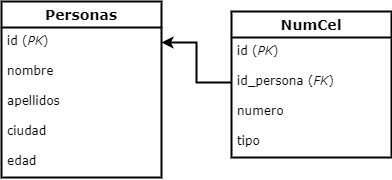
\includegraphics[width=8cm]{ss/relacion_tablas.jpg}
\end{figure}

Ambas tablas tienen su llave primaria junto con sus registros, pero la tabla "NumCel" tiene una columna llamada "id\_persona" que contiene los ids de las personas de la columna "id" de la tabla "Personas", por lo que esta columna es la que realmente hace la relación entre ambas columnas; la llave foránea de una tabla es la que conecta con la llave primaria de la otra tabla.

El comando \textbf{FOREIGN KEY ()} permite asignar la llave foránea de una tabla a una columna, analicemos el siguiente comando:
\begin{lstlisting}
    FOREIGN KEY (customer_id) REFERENCES Personas(id)
\end{lstlisting}

\textit{FOREIGN KEY (customer\_id)} asigna la llave foránea a la columna "customer\_id" de la tabla "NumCel", y \textit{REFERENCES Personas(id)} es la llave primaria de la tabla a relacionar, es aquí donde se crea la relación (en código) de ambas tablas. Insertamos algunos registros en la tabla "NumCel" y veamos visualmente como se ve el resultado en la \textit{Figura \ref{fig: 2}}:
\begin{figure}[H]
    \centering
    \caption{Tablas relacionadas}
    \label{fig: 2}
    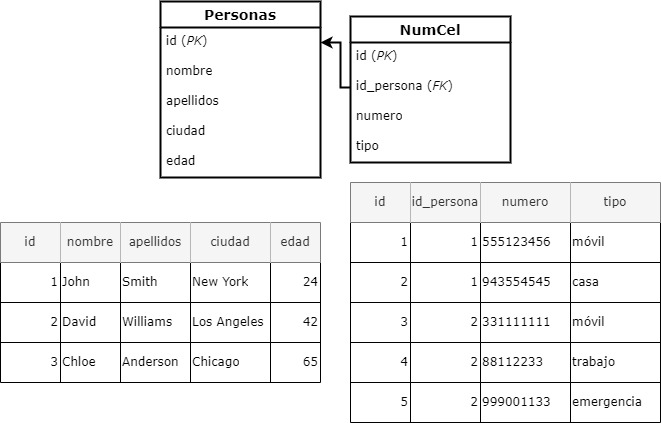
\includegraphics[width=11cm]{ss/tablas_relacionadas.jpg}
\end{figure}

\textit{Nota}: una tabla puede tener múltiples llaves foráneas.



\section{Llaves Únicas}

Las \textbf{llaves únicas} (\textbf{UNIQUE}) son columnas que poseen valores únicos (no duplicados) pero no son el identificador ni llave primaria de la tabla, una tabla puede tener varias llaves únicas, pero una sola llave primaria. Haremos que la columna "apellidos" de la tabla "Personas" sea una llave única:
\begin{lstlisting}
    ALTER TABLE Personas
    ADD UNIQUE apellidos
\end{lstlisting}

Ahora, cada apellido de cada registro no podrá estar duplicado, por lo que si intentamos insertar un registro con el apellido "Anderson" u alguno otro de esta tabla tendremos un error. Los valores \textit{NULL} son ignorados en una llave única, por lo que podemos tener múltiples valores NULL en estas columnas.

\section{Múltiples tablas}

En el mundo real, existen miles de registros en una tabla, y un registro puede estar conectado con otra tabla, como en el ejemplo anterior de las personas y los números de celular.

El comando \textit{SELECT, FROM y WHERE} permiten consultar información de dos tablas en una misma sentencia (\textit{Tabla \ref{tab: 32}}):
\begin{lstlisting}
    SELECT nombre, apellidos, ciudad, numero, tipo
    FROM Personas, NumCel
    WHERE Personas.id = NumCel.id_personas
\end{lstlisting}
\begin{table}[H]
    \centering
    \caption{Sentencia usando dos tablas}
    \label{tab: 32}
    \begin{tabular}{|l|l|l|l|l|}
        \hline
        \textbf{nombre} & \textbf{apellidos} & \textbf{ciudad} & \textbf{numero} & \textbf{tipo} \\
        \hline
        John    & Smith     & New York      & 555123456 & móvil \\
        \hline
        John    & Smith     & New York      & 943554545 & casa \\
        \hline
        David   & Williams  & Los Angeles   & 331111111 & móvil \\
        \hline
        David   & Williams  & Los Angeles   & 88112233  & trabajo \\
        \hline
        David   & Williams  & Los Angeles   & 999001133 & emergencia \\
        \hline
    \end{tabular}
\end{table}

Utilizar [nombre de tabla].[llave primaria] y [nombre de tabla].[llave foránea] es recomendable para hacer sentencias con más de una tabla, esto hace que las sentencias sean más fáciles de leer, este mismo formato aplica para consultas de una sola tabla:
\begin{center}
    \textit{SELECT PERSONAS.edad FROM Personas}
\end{center}

El siguiente ejemplo es igual a un \textit{SELECT * FROM Personas, NumCel} y muestra simplemente el uso del formato citado anteriormente:
\begin{lstlisting}
    SELECT Personas.nombre, Personas.apellidos, Personas.ciudad, Personas.edad, NumCel.numero, NumCel.tipo
    FROM Personas, NumCel
    WHERE Personas.id = NumCel.id_personas
\end{lstlisting}



\section{JOIN}

Otra forma de combinar dos tablas en una consulta es por medio del comando \textbf{JOIN}, este comando funciona en base en condiciones, utilizaremos el ejemplo del tema anterior pero con \textit{JOIN}:
\begin{lstlisting}
    SELECT nombre, apellidos, ciudad, numero, tipo
    FROM Personas JOIN NumCel
    ON Personas.id = NumCel.id_personas
\end{lstlisting}

\textit{FROM Personas JOIN NumCel} hace la unión entre ambas tablas y \textit{ON} establece la condición. Este comando tiene el aspecto de la \textit{Figura \ref{fig: 3}}:
\begin{figure}[H]
    \centering
    \caption{Concepto de JOIN}
    \label{fig: 3}
    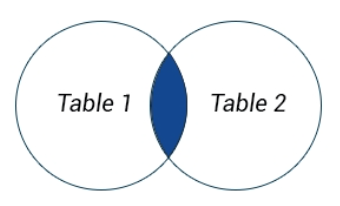
\includegraphics[width=5cm]{ss/join.png}
\end{figure}

Los registros relacionados por la condición de \textit{ON} en ambas tablas aparecen en la zona coloreada.


\subsection{Alias}

En el ejemplo donde recogemos todos los registros de todas las columnas, utilizamos el formato [nombre de tabla].[columna] el cual puede terminar siendo muy largo, es entonces que podemos abreviar el nombre de las columnas a una o pocos caracteres de la siguiente manera:
\begin{lstlisting}
    SELECT P.nombre, P.apellidos, P.ciudad, NC.numero, NC.tipo
    FROM Personas AS P JOIN NumCel AS NC
    ON C.id = NC.id_personas
\end{lstlisting}

Abreviamos el nombre de las tablas en el \textit{SELECT} y definimos esta abreviación con \textit{AS} en el \textit{FROM}, a esto se le llama \textbf{alias de tablas}.


\subsection{Tipos de JOIN}

\textit{JOIN} selecciona los registros que coinciden en ambas tablas, \textbf{LEFT JOIN} selecciona los registros que coinciden en ambas tablas y los de la primer tabla (tabla izquierda), el aspecto de \textit{LEFT JOIN} está en la \textit{Figura \ref{fig: 4}}:
\begin{figure}[H]
    \centering
    \caption{Concepto de LEFT JOIN}
    \label{fig: 4}
    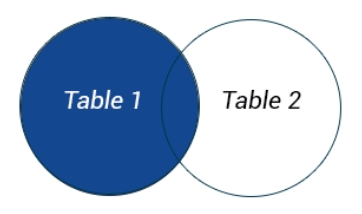
\includegraphics[width=5cm]{ss/left_join.png}
\end{figure}

\textbf{RIGHT JOIN} selecciona los registros que coinciden en ambas tablas y los de la segunda tabla (tabla derecha).



\section{UNION}

Este comando permite combinar los registros de ambas tablas; si en estas tablas hay dos o más registros iguales entre si (duplicados), solo se agrega uno de ellos y no sus duplicados.

Para combinar correctamente los registros, en la sentencia debe haber el mismo número de columnas, tipo de dato y que el orden de las columnas sea el mismo. Para ejemplificar este comando, partiremos la tabla "Personas" en dos y duplicaremos algunos registros, quedando como resultado las siguientes \textit{Tablas}:
\begin{table}[H]
    \centering
    \caption{Tabla "Personas" a la mitad}
    \label{tab: 33}
    \begin{tabular}{|l|l|l|l|l|}
        \hline
        \textbf{id} & \textbf{nombre} & \textbf{apellidos} & \textbf{ciudad} & \textbf{edad} \\
        \hline
        1 & John        & Smith     & New York      & 24 \\
        \hline
        2 & David       & Williams  & Los Angeles   & 42 \\
        \hline
        3 & Chloe       & Anderson  & Chicago       & 65 \\
        \hline
        4 & Emily       & Adams     & Houston       & \textit{NULL} \\
        \hline
        5 & James       & Roberts   & Philadelphia  & 31 \\
        \hline
        6 & John        & Smith     & New York      & 24 \\
        \hline
        7 & David       & Williams  & Los Angeles   & 42 \\
        \hline
    \end{tabular}
\end{table}
\begin{table}[H]
    \centering
    \caption{Tabla "Contactos"}
    \label{tab: 34}
    \begin{tabular}{|l|l|l|l|l|}
        \hline
        \textbf{id} & \textbf{nombre} & \textbf{apellidos} & \textbf{ciudad} & \textbf{edad} \\
        \hline
        1 & Andrew      & Thomas    & New York      & 21 \\
        \hline
        2 & Daniel      & Harris    & New York      & 67 \\
        \hline
        3 & Charlotte   & Walker    & Chicago       & \textit{NULL} \\
        \hline
        4 & Samuel      & Clark     & San Diego     & \textit{NULL} \\
        \hline
        5 & Anthony    & Young     & Los Angeles   & 52 \\
        \hline
        6 & Daniel      & Harris    & New York      & 67 \\
        \hline
        7 & Samuel      & Clark     & San Diego     & \textit{NULL} \\
        \hline
    \end{tabular}
\end{table}

El siguiente ejemplo con \textit{UNION} dará como resultado la \textit{Tabla \ref{tab: 35}}:
\begin{lstlisting}
    SELECT id, nombre, apellidos, ciudad, edad FROM Personas
    UNION
    SELECT id, nombre, apellidos, ciudad, edad FROM Contactos
\end{lstlisting}
\begin{table}[H]
    \centering
    \caption{Unión de las tablas "Personas" y "Contactos"}
    \label{tab: 35}
    \begin{tabular}{|l|l|l|l|l|}
        \hline
        \textbf{id} & \textbf{nombre} & \textbf{apellidos} & \textbf{ciudad} & \textbf{edad} \\
        \hline
        1 & John        & Smith     & New York      & 24 \\
        \hline
        2 & David       & Williams  & Los Angeles   & 42 \\
        \hline
        3 & Chloe       & Anderson  & Chicago       & 65 \\
        \hline
        4 & Emily       & Adams     & Houston       & \textit{NULL} \\
        \hline
        5 & James       & Roberts   & Philadelphia  & 31 \\
        \hline
        6 & Andrew      & Thomas    & New York      & 21 \\
        \hline
        7 & Daniel      & Harris    & New York      & 67 \\
        \hline
        8 & Charlotte   & Walker    & Chicago       & \textit{NULL} \\
        \hline
        9 & Samuel      & Clark     & San Diego     & \textit{NULL} \\
        \hline
        10 & Anthony    & Young     & Los Angeles   & 52 \\
        \hline
    \end{tabular}
\end{table}

Este ejemplo utiliza dos tablas con la misma cantidad de columnas del mismo tipo, muestra todos los registros de ambas tablas menos los registros duplicados. El comando \textbf{UNION ALL} si incluye registros duplicados. En caso de que queramos unir dos tablas, pero alguna de ellas tiene columnas extras que queramos unir, podemos agregar dicha columna en alguna de las sentencias \textit{SELECT}, en el siguiente ejemplo ponemos una columna llamada "trabajo" que solamente existe en la tabla "Contactos" (\textit{Tabla \ref{tab: 36}}):
\begin{lstlisting}
    SELECT id, nombre, apellidos, ciudad, edad, trabajo FROM Contactos
    UNION
    SELECT id, nombre, apellidos, ciudad, edad, NULL FROM Personas
\end{lstlisting}
\begin{table}[H]
    \centering
    \caption{Union de las tablas "Personas" y "Contactos"}
    \label{tab: 36}
    \begin{tabular}{|l|l|l|l|l|l|}
        \hline
        \textbf{id} & \textbf{nombre} & \textbf{apellidos} & \textbf{ciudad} & \textbf{edad} & \textbf{trabajo} \\
        \hline
        1 & John        & Smith     & New York      & 24            & ingeniero \\
        \hline
        2 & David       & Williams  & Los Angeles   & 42            & \textit{NULL} \\
        \hline
        3 & Chloe       & Anderson  & Chicago       & 65            & licenciada \\
        \hline
        4 & Emily       & Adams     & Houston       & \textit{NULL} & \textit{NULL} \\
        \hline
        5 & James       & Roberts   & Philadelphia  & 31            & \textit{NULL} \\
        \hline
        6 & Andrew      & Thomas    & New York      & 21            & \textit{NULL} \\
        \hline
        7 & Daniel      & Harris    & New York      & 67            & ingeniero \\
        \hline
        8 & Charlotte   & Walker    & Chicago       & \textit{NULL} & \textit{NULL} \\
        \hline
        9 & Samuel      & Clark     & San Diego     & \textit{NULL} & \textit{NULL} \\
        \hline
        10 & Anthony    & Young     & Los Angeles   & 52            & licenciado \\
        \hline
    \end{tabular}
\end{table}

Al tener la primer sentencia \textit{SELECT} una columna extra, la segunda debe tener una columna extra para que sean el mismo número de columnas con el mismo tipo de dato, en este caso, asignamos una columna con solamente valores \textit{NULL}.

Podemos utilizar condiciones dentro de las uniones:
\begin{lstlisting}
    SELECT id, nombre, apellidos, ciudad, edad FROM Personas
    WHERE edad > 30
    UNION
    SELECT id, nombre, apellidos, ciudad, edad FROM Contactos
    WHERE edad < 25
\end{lstlisting}


% Fin del documento.
\end{document}